\documentclass[aps,prl,twocolumn,superscriptaddress,floatfix]{revtex4-2}

\usepackage{amsmath,amssymb}
\usepackage{graphicx}
\usepackage{hyperref}
\usepackage{xcolor}

\begin{document}

\title{Strange Attractors in Gradient Descent: Data Structure and Loss Geometry Control Fractal Dimension}

\author{Evan Paul}
\email{evan@evanpaul.us}
\affiliation{Independent Researcher}

\date{\today}

\begin{abstract}
We measure the correlation dimension $D_2$ of neural network training trajectories in function space. Under full-batch gradient descent, networks trained on CIFAR-10 produce strange attractors whose dimension converges to $D_2 \approx 5$ at long trajectory lengths (conservative lower bounds from shorter trajectories: $3.67 \pm 0.08$ for a CNN, $4.4$--$4.6$ for MLPs). Cross-architecture controls show structured data is necessary for multi-dimensional chaos---either architecture on synthetic data gives $D_2 \approx 1$---while architecture modulates the learning-rate threshold. A label-noise sweep reveals regime-dependent control: at moderate learning rates, degrading labels reduces $D_2$ from $3.6$ to $2.3$; near the Edge of Stability, loss-surface roughness sustains high-dimensional dynamics independently. The attractor survives stochastic gradient descent, retaining $>$82\% of its fractal dimension at $20\times$ gradient noise.
\end{abstract}

\maketitle

\section{Introduction}

Gradient descent is a deterministic dynamical system. Each update maps the network's function to a new function, tracing a trajectory through function space. Recent work shows this trajectory is rich: Edge of Stability oscillations~\cite{cohen2021,damian2023}, period-doubling cascades~\cite{kalra2025,ghosh2025}, positive Lyapunov exponents~\cite{morales2024,storm2024}. These confirm chaos. They do not tell us its shape. We measure the correlation dimension $D_2$~\cite{grassberger1983} and find strange attractors shaped by two mechanisms: structured data creates oscillatory modes at moderate learning rates; loss-surface roughness sustains chaos near the Edge of Stability.

\section{Methods}

Five conditions under full-batch gradient descent, MSE loss, no momentum or weight decay (Table~\ref{tab:conditions}): a CNN (268K parameters) and two MLPs (156K, 269K) on 2{,}000 CIFAR-10 images, plus CNN and MLP controls on synthetic data (i.i.d.\ Gaussian inputs in 220 dimensions, 10 classes with randomly assigned labels---no geometric or statistical structure in either the inputs or the input-label mapping). By ``structured data'' we mean inputs whose distribution has low-dimensional geometric structure and whose labels reflect learnable correlations with that structure, as in natural images; the synthetic control is designed to lack both properties. Learning rates span 5--95\% of $2/\lambda_{\max}$ (EoS threshold after 1{,}000 warmup steps). All runs: 5{,}000 steps. Full architectural details in~\cite{sm}.

Chaos is measured in function space to avoid gauge artifacts from overparameterization. Two model copies train from identical initialization, one perturbed by $\varepsilon = 10^{-5}$ along a random direction. The divergence rate $\lambda$ is the slope of $\ln\lVert f(\mathbf{x}) - \tilde{f}(\mathbf{x})\rVert$ on 100 held-out inputs over $[0.2T, 0.8T]$. This is a finite-scale rate; sensitivity analysis~\cite{sm} confirms $\varepsilon \geq 10^{-6}$ is required---smaller values produce uniform numerical artifacts. The $\varepsilon$-dependence implies systematic uncertainty of roughly $3\times$ beyond seed-to-seed variability. Results: 10 seeds (CIFAR-10 conditions), 20 seeds (MLP/synthetic).

$D_2$ is computed via Grassberger-Procaccia~\cite{grassberger1983} on ${\sim}400$ function-space trajectory points (outputs every 10 steps, first 20\% discarded). Calibration on 11 known dynamical systems~\cite{sm} shows 15--35\% systematic underestimate for fractal attractors; all reported values are conservative lower bounds. Persistent homology (\textsc{ripser}~\cite{ripser}) provides independent topological confirmation.

\begin{figure*}[t]

\includegraphics[width=\textwidth]{figures/cifar10_eos.png}
\caption{\label{fig:cnn}%
CNN on CIFAR-10, 10 seeds.
(a)~$\lambda$ versus EoS fraction. Peaks at 15\%, crosses zero near 45\%.
(b)~$D_2$ versus EoS fraction. Peaks at $3.67 \pm 0.08$ at 30\%.
(c)~Second principal component variance.
(d)~Sharpness: progressive at 5\% EoS versus bounded oscillation at 95\%. Error bars: standard deviation.}
\end{figure*}

\section{Results}

\textit{Chaos window.}---$\lambda$ is non-monotonic [Fig.~\ref{fig:cnn}(a)]. For the CNN on CIFAR-10, it peaks at 15\% of EoS and crosses zero near 45\%. Above this, basin convergence dominates. The bounded window appears in every architecture.

\textit{Strange attractors.}---Within the window, trajectories acquire fractal structure [Fig.~\ref{fig:cnn}(b)]. $D_2$ crosses 1.0 at 10\% EoS, peaks at $3.67 \pm 0.08$ at 30\%, remains above 2.0 to 80\%. The first principal component captures only 52\% of variance. A convergence analysis at $N = 3{,}200$~\cite{sm} shows $D_2$ has not saturated: both MLPs stabilize near 5.1. Accounting for calibration bias, true dimensions likely lie in the range 4--7. Persistent homology confirms fractal topology across all architectures~\cite{sm}: hundreds of $H_1$ features at all scales, gap ratio near 1.0---no dominant structure.

\textit{Data is necessary; architecture sets the threshold.}---The controls (Table~\ref{tab:conditions}, Fig.~\ref{fig:cross}) separate cleanly. CNN on synthetic data: $D_2 < 1$ at all learning rates. Both MLPs on CIFAR-10: $D_2 > 4$ at 90\% EoS, converging to ${\sim}5.1$. Structured data is necessary and sufficient for multi-dimensional chaos. The CNN reaches $D_2 = 3.67$ at 30\% EoS; the MLPs need 70--90\%.

\textit{Two mechanisms.}---A label-noise sweep from clean ($p = 0$) to random labels ($p = 1$) at each architecture's peak (Fig.~\ref{fig:noise}) reveals two regimes. CNN at 30\% EoS: $D_2$ falls monotonically from $3.64 \pm 0.08$ to $2.34 \pm 0.75$---degrading labels weakens the modes. MLP at 90\% EoS: $D_2$ rises from $4.38 \pm 0.07$ to $4.70 \pm 0.09$---random labels roughen the loss surface, sustaining chaos through competing minima. The sign of $D_2$'s response to label noise reverses across regimes. Notably, even at $p = 1$ the CNN on CIFAR-10 retains $D_2 = 2.34$, well above the CNN/synthetic baseline ($D_2 \approx 1$), indicating that the geometric structure of the inputs contributes independently of label information.

\textit{Robustness.}---A batch-size sweep from $B = 2{,}000$ to $B = 100$~\cite{sm} shows graceful degradation: the CNN retains 87\% and the MLP 82\% of full-batch $D_2$, both remaining above 3.0. Meanwhile $\lambda$ increases $10\times$---SGD amplifies sensitivity along existing modes without creating new dimensions.

\textit{Dissociation.}---Peak $\lambda$ and peak $D_2$ occur at different learning rates in every architecture (CNN: 15\% vs 30\%; MLPs: 40--50\% vs 90\%). Geometric complexity peaks not at maximum sensitivity but where chaotic and convergent dynamics compete.

\begin{figure}[t]
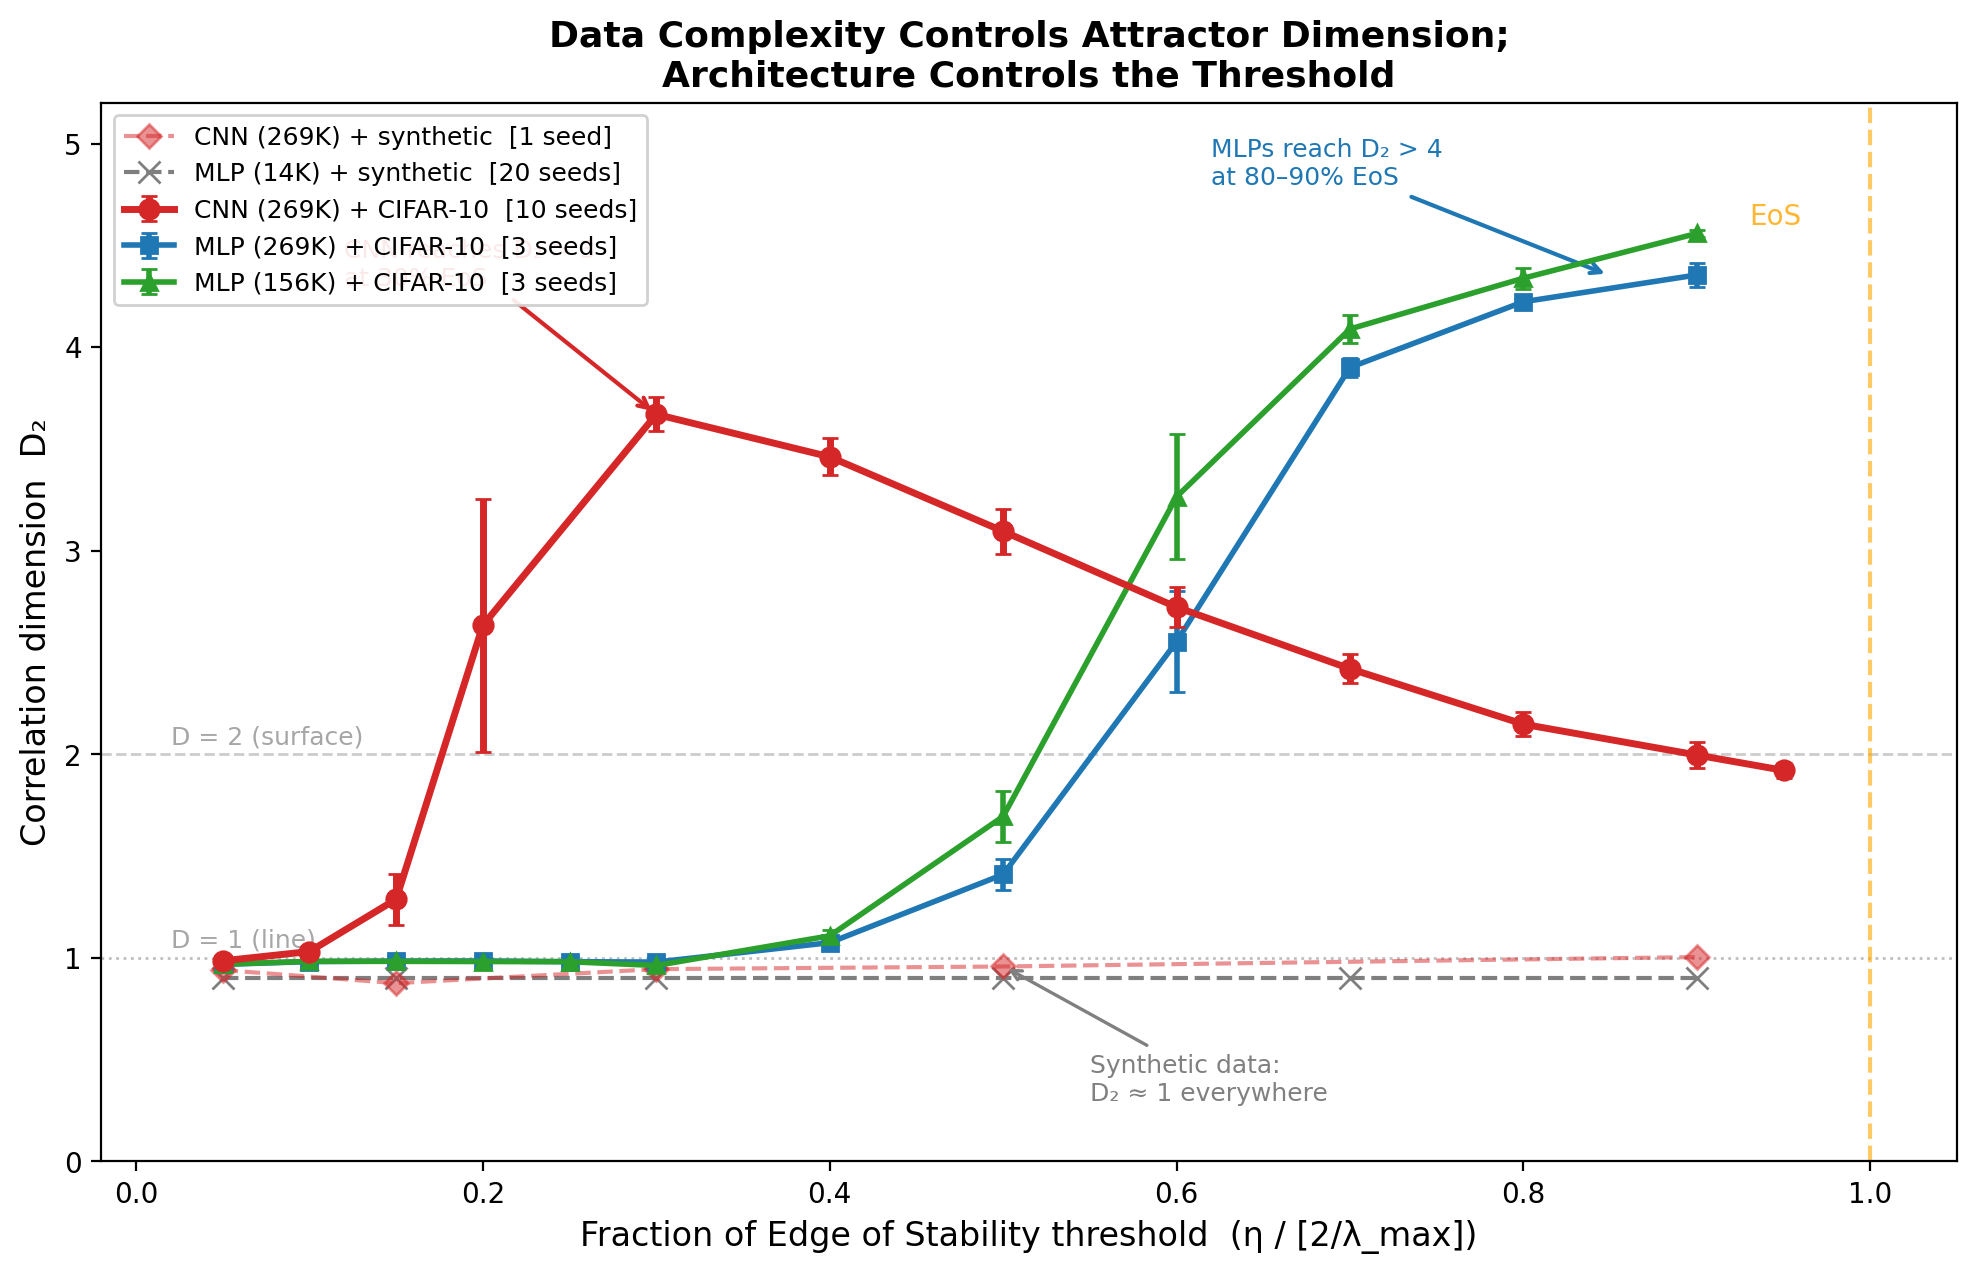
\includegraphics[width=\columnwidth]{figures/figure2_cross_experiments.png}
\caption{\label{fig:cross}%
$D_2$ versus EoS fraction, all five conditions. CIFAR-10 (filled markers): $D_2 > 3$. Synthetic (open): $D_2 \approx 1$ throughout. Error bars: standard deviation.}
\end{figure}

\begin{figure}[t]

\includegraphics[width=\columnwidth]{figures/revision1/label_noise_d2.pdf}
\caption{\label{fig:noise}%
$D_2$ versus label-noise fraction $p$. CNN at 30\% EoS (red): $D_2$ falls. MLP~269K at 90\% EoS (blue): $D_2$ rises. Seven seeds; error bars show standard deviation. Note that CNN error bars above $p = 0.5$ are large ($\sigma/\mu \approx 30\%$); the monotone trend is robust but the precise functional form is underdetermined at high noise.}
\end{figure}

\begin{table}[b]
\caption{\label{tab:conditions}%
Peak $D_2$ for each condition. $N{=}3200$ column: converged values~\cite{sm}. The CNN/CIFAR converged value ($^*$) is from a single seed and is noisier than the MLP conditions.}
\begin{ruledtabular}
\begin{tabular}{lcccccc}
 & & & \multicolumn{2}{c}{$D_2$} & & \\
\cline{4-5}
 & Params & Data & $N{\approx}400$ & $N{=}3200$ & EoS\% & Seeds\\
\hline
MLP/synth. & 14K & synth. & 0.9 & --- & all & 20\\
CNN/synth. & 269K & synth. & $0.98(3)$ & --- & 90 & 10\\
MLP/CIFAR & 156K & C-10 & $4.61(10)$ & ${\sim}5.1$ & 90 & 10\\
MLP/CIFAR & 269K & C-10 & $4.37(5)$ & ${\sim}5.1$ & 90 & 10\\
CNN/CIFAR & 269K & C-10 & $3.67(8)$ & ${\sim}5^*$ & 30 & 10\\
\end{tabular}
\end{ruledtabular}
\end{table}

\section{Discussion}

The phenomenology is suggestive of classical routes to chaos~\cite{ruelle1971,newhouse1978}: structured data creates oscillation axes; coupling through training dynamics produces a strange attractor. We note, however, that gradient descent is dissipative and non-Hamiltonian, so frameworks such as KAM theory or the Newhouse-Ruelle-Takens route apply only as phenomenological analogies---the sequential appearance of independent quasi-periodic modes has not been demonstrated here. The CNN's hierarchy lowers the coupling threshold; the MLP reaches the same destination with harder driving. Without structured data, the modes do not exist. That $D_2$'s response to label noise reverses sign across regimes---falling at 30\% EoS, rising at 90\%---is a constraint on any theoretical account. A complete picture likely involves three factors: label structure (which creates modes at moderate learning rates), loss-surface roughness (which sustains chaos near the EoS), and input geometry (which contributes independently, as evidenced by $D_2 = 2.34$ for the CNN at $p = 1$ versus $D_2 \approx 1$ on synthetic inputs). These dynamical findings complement the static toroidal topology identified by Pittorino \textit{et al.}~\cite{pittorino2022}.

A methodological caution: our $\lambda$ values are finite-scale rates, not true Lyapunov exponents. At $\varepsilon = 10^{-8}$, measurements are dominated by numerical noise~\cite{sm}; prior work at smaller $\varepsilon$~\cite{morales2024} should be interpreted carefully. Storm \textit{et al.}~\cite{storm2024} measured finite-time Lyapunov exponents in weight space; such measurements are susceptible to gauge artifacts from weight-space symmetries (permutation, rescaling) that can inflate apparent divergence rates without reflecting genuine dynamical sensitivity of the network's input-output map. Our function-space protocol avoids these false positives.

The learning rates that produce strange attractors overlap with practice~\cite{cohen2021}. Whether the attractor matters---whether exploring it produces better solutions---is the question these measurements now enable.

\begin{acknowledgments}
AI language models (Claude, Anthropic) were used as research tools throughout this work: code co-development (training loops, analysis pipelines), literature identification, and iterative manuscript drafting. The research question, experimental design decisions, choice of measurements, interpretation of results, and all scientific conclusions are the author's sole responsibility. Code, data, and scripts: \url{https://github.com/gnomevan/attractor}.
\end{acknowledgments}

\bibliography{references}

\end{document}
